\documentclass{article}
\usepackage{graphicx}
\graphicspath{{images/}}

\begin{document}
	\title{Image Classification Report}
	\author{Rowan Powell rp9g14\\Stewart Paterson sp16g14\\Bradley Mason bm6g14}
	\maketitle
	\newpage
	\section{Image Augmentation}
	
	\subsection{Purpose}
	For our image classification software we do not have a particularly large dataset to train upon which limits the effectiveness of the training and how generalisable the results are for unseen data. The concept employed is to create a significantly larger dataset, in this case by a factor of 5, where permutations of the original image set cause the classifier to learn the general properties of classes of images rather than the features specific to the dataset it is trained upon.
	
	\begin{figure}[h]
		\centering
		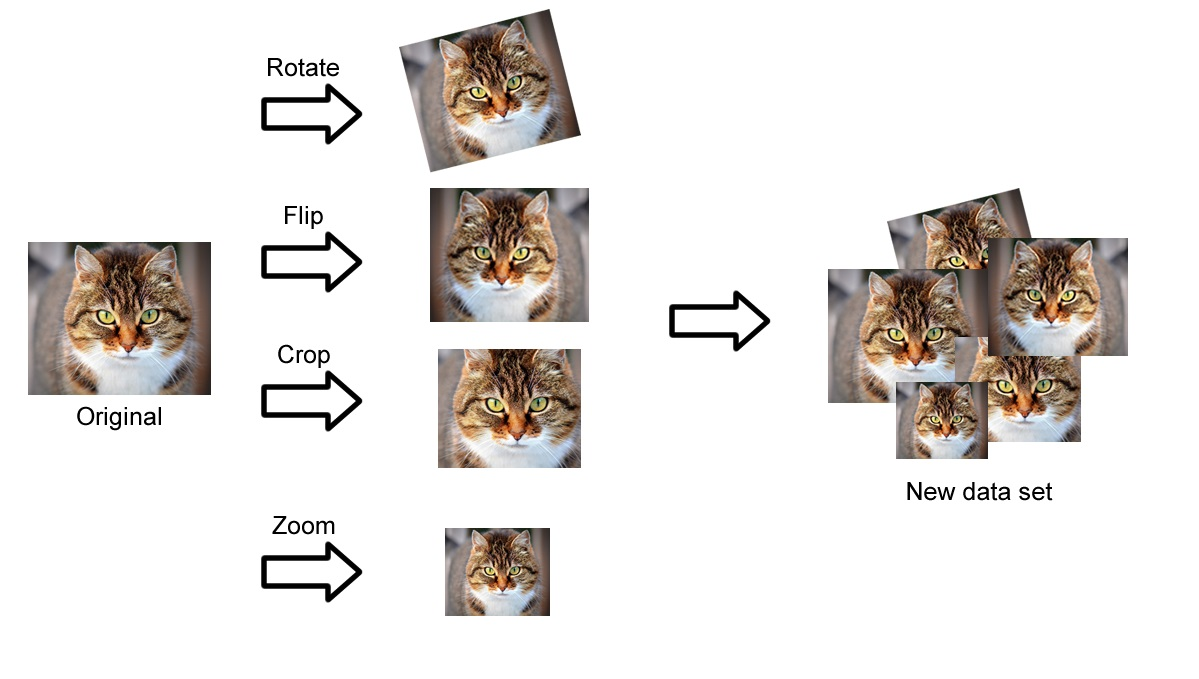
\includegraphics[scale=0.3]{augment}
		\caption{Image Augmentation Structure Diagram}
	\end{figure}
	
	\subsection{Process}
	We wrote a short program that finds all of the folders containing images within the training directory and populates those with augmented variants. A slightly rotated image is created, keeping the general orientation of the image but introducing some slight rotation invariance into the image. Secondly a horizontally flipped image is created to help generalise for lighting and perspectives within the data set. A cropped image is created that removes up to 20\% of the original image from the edges to encourage the classifier to identify the class from subsets of features within the image. We create a slightly (up to 25\%) zoomed in or out image to promote identification of key features at various sizes.
	
	
	\section{Run 1}
	
	\subsection{Introduction}
	For run 1 we were asked to develop a K nearest neighbour classifier that used the tiny image feature extractor.
	\subsection{TinyImage Feature}
	We have a class that implements the \textit{FeatureExtractor} interface, then the \textit{extractFeature} method for producing the tiny image.
	This method takes an image as input, it crops the image square and then resizes it to become a 16x16 pixel image using the OpenIMAJ \textit{ResizeProcessor} library.
	The next task was to make the image zero mean and unit length. I achieved this by using the \textit{FImage} class to find the sum of the pixels and therefore the mean. I then had to find the variance which I could not find a method for, so I loop through the pixels in the image and cumulatively calculate the variance, from which I could calculate the standard deviation.
	I then used the \textit{FImage} class to \textit{subtractInPlace} and \textit{divideInPlace} in order to make the image zero mean and unit length. Finally I use \textit{FImage} to convert the image into a single dimension vector and return it as a \textit{FloatFV} object.
	\subsection{KNN}
	In my main Run1 class I then implement this. I fetch the training and testing images and split the training images 450:50 for training:testing. I am able to have a training sample this high thanks to the \textit{ImageAugmenter} class we wrote that modifies the training images to increase our resources.
	I have an \textit{evaluateK} method that trains a \textit{KNNAnnotator} using the \textit{TinyImage} feature vector with the 450 sample, it then tests this for values of K from 1-9. It tests it 5 times with the remaining 50 testing images to collect the accuracy and finds the average. The highest average accuracy K value is then returned.\\
	\begin{tabular}{|c|c|}
		\hline
		K-Value & Accuracy\\ \hline \hline
		1 & 0.65\\
		2 & 0.597\\
		3 & 0.553\\
		4 & 0.505\\
		5 & 0.457\\
		6 & 0.425\\
		7 & 0.391\\
		8 & 0.368\\
		9 & 0.339\\ \hline
	\end{tabular}
	
	I tested this and found a K of 1 to be the most accurate so I implemented this manually in my code to save time, although I have a commented line that will choose the K using the aforementioned method.
	A new \textit{KNNAnnotator} is then set up with the optimal K and trained using the same 450 training data. I then start a \textit{PrintWriter} and iterate through the testing images provided for the spec, writing to a file the name of the image file and the class that the classifier has predicted.
	Finally I close the \textit{PrintWriter} and the application ends.
	\section{Run 2}
	
	Run 2 takes a series of densely sampled pixel patches from each image, converts them into feature vectors by taking the pixel values within the patch, and classifies them into a set of visual words. From there, a histogram of visual words is generated for each image, and a set of one-versus-all classifiers are generated using a \textit{LiblinearAnnotator} to classify the images. 
	
	\subsection{ Histogram of Visual Words }
	
	I first wrote a method which extracts a List of feature vectors based on the densely sampled pixel patches within an image. It loops through each pixel patch, and calculates the corresponding feature vector. It also normalises each vector before returning, by subtracting the mean of all values in the vector, and dividing by the standard deviation.\\
	In order to generate the set of visual words, I take a random sample of 40,000 vectors from analysing the training dataset, and run K-Means on it, with a K value of 500. The list of centroids then forms the set of visual words.\\
	\newline
	
	I wrote a class implementing the \textit{FeatureExtractor} interface which produces a histogram of the frequency of the visual words for a given \textit{FImage}. It first generates the list of feature vectors for the image, then uses a \textit{HardAssigner} to classify them into visual words, and construct a histogram of the frequency of each word.
	
	\subsection{ LibLinear Annotator }
	
	Once I have created a \textit{FeatureExtractor} based on the generated set of visual words, I train a \textit{LiblinearAnnotator} to classify the training data based on the histogram of words produced by each training image. The \textit{LiblinearAnnotator} uses a series of one-versus-all classifiers to classify the image into one of the classes, based on the histogram produced by the \textit{FeatureExtractor}.
	
	\subsection{ Accuracy }
	
	I did some test runs on a small amount of data in order to find what the good values for the size of the patches, interval between the patches, and how many samples on which to run K-Means. I found that good values were a patch size of $7\times7$, at intervals of 4, and using  a sample size of 40,000 for running K-Means. \\
	\\
	I performed a final run using 450 training images per class from the augmented data, and evaluated its performance against a labelled testing set of 50 images per class. This achieved an accuracy of 70.3\%. I then ran the classifier on the unlabelled test data and outputted its results to a file.\\
	\\Results with Variable Training Sample Size\\
	\begin{tabular}{|c|c|}
		\hline
		Training Sample Size & Accuracy(binsize=7,stepsize=4)\\ \hline \hline
		10,000 & 0.5420 \\
		20,000 & 0.5820 \\
		30,000 & 0.6072 \\
		40,000 & 0.6178 \\
		50,000 & 0.6088 \\ \hline
	\end{tabular}\\
	Result with Variable Bin Size\\
	\begin{tabular}{|c|c|}
		\hline
		Bin Size & Accuracy(stepsize=4,trainingSampleSize=40000)\\ \hline \hline
		5 & 0.5696 \\
		6 & 0.5396 \\
		7 & 0.5958 \\
		8 & 0.5788 \\
		9 & 0.5706 \\ \hline
	\end{tabular}\\
	Results with Variable Step Size\\
	\begin{tabular}{|c|c|}
		\hline
		Step Size & Accuracy(binsize=7,trainingSampleSize=40000)\\ \hline \hline
		2 & 0.5913 \\
		3 & 0.5897 \\
		4 & 0.5987 \\
		5 & 0.5673 \\
		6 & 0.56 \\ \hline
	\end{tabular}
	
	\section{Run 3}
	In summary Run 3 sets up a Pyramid Dense SIFT feature extractor and trains it using a KNN algorithm, all from the OpenIMAJ library. It then creates, trains and evaluates each of our classifiers. We have three, it then evaluates once more with each of the trained classifiers predicting the class of each image and voting with weighting based on accuracy. Finally the code iterates through the test images provided, the classifiers each vote for a class and writes the voted class of each to a text file.\\
	Originally we had four voting classifier however in testing it became apparent that the linear SVM was much less accurate than other classifiers so we thought it was worth removing from the algorithm.
	
	\begin{figure}[h]
		\centering
		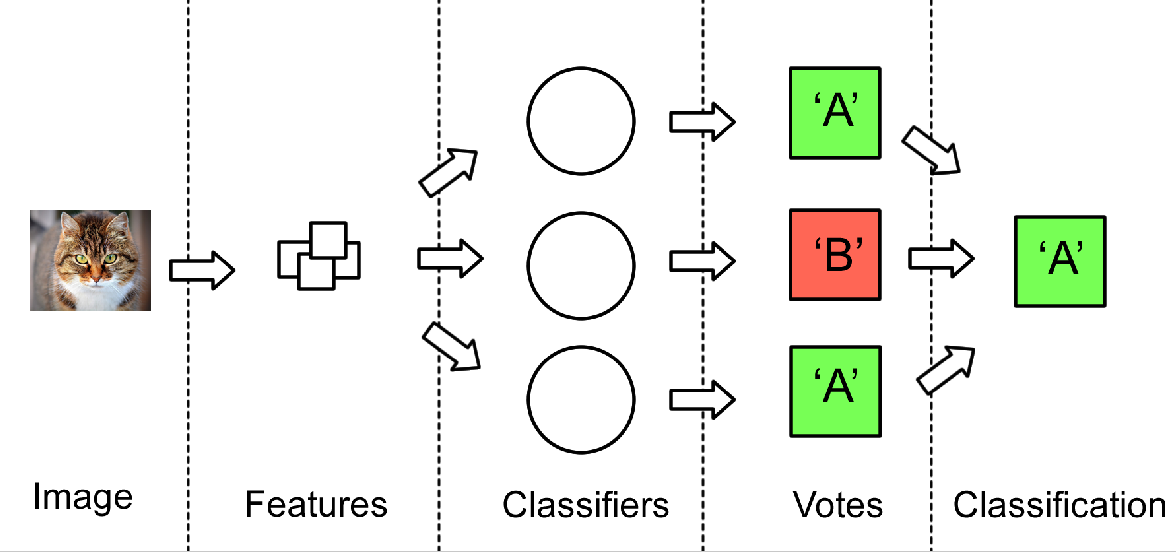
\includegraphics[scale=0.4]{structure}
		\caption{Overall Run 3 Structure Diagram}
	\end{figure}
	
	\subsection{Main Class}
	The Run 3 main class organises the other methods. Initially it produces the \textit{ClassificationVoteAggregator} and passes it the testing and training data.\\
	It also contains a small evaluation class that, using training data, gets the predicted class from the voting between the classifiers and compares it to the answer. This then produces our accuracy value for the entire run.\\
	The real work now begins when we iterate through the provided testing images, keeping track of the file name and fetching the predicted class for each image. The result is then stored in a text file.\\
	The collate votes method is the method that takes an image, passes it to each of the classifiers and then proceeds with a simple voting system that votes for the most likely class. It returns the result.
	
	\subsection{ClassificationVoteAggregator}
	This class is the backbone of run 3. When an instance is created it uses a method to produce the feature extractor, this extractor consists of a KNN trained pyramid dense SIFT that applies the bag of visual words model with a block spatial aggregator and then wraps this in a homogeneous kernel map. This part is all done with classes straight from the OpenIMAJ library.
	\newline
	
	It then creates a new classifier from the interface \textit{Classifier} and passes them the generated extractor. We have produced a Lib Linear classifier, a Naive Bayes classifier, a linear SVM classifier and a densely sampled pixel patch classifier.
	\newline
	
	We then train each of these using training data from the training images provided, plus the additional augmented images. We also then evaluate each of these classifiers using a portion of the testing images, we varied the split but found that the best performance value is a feasible time was 200:50 for training:testing. When each of the classifiers is evaluated it stores it's own accuracy for later use as a weight. This class also has a get votes method which takes an image as input and uses each of the classifiers and returns a hash map of the voted class and the weight as a percentage represented as the number of votes.
	
	\subsection{Classifier}
	We developed a classifier interface such that we could then implement instances of this in the code.\\
	The get vote and evaluate methods remain the same throughout so these are defined in the classifier interface, the constructor and train methods are implementation dependent so these are left to the implemented classes to implement.
	
	\subsection{DenselySampledPixelPatches}
	This class is an adaption of the code from Run 2 that has been made to suit the remainder of Run 3, we are using this as a fourth classifier.
	
	\subsection{The Result}
	We launched run 3 with the highest parameters we could afford to wait for and had the memory for. We changed the training:testing split to 150:50, which produced the following results:\\
	\\
	\begin{tabular}{|c|c|}
		\hline
		\textbf{Classifier} & \textbf{Evaluated Accuracy}\\ \hline
		Lib Linear & 0.881\\
		Naive Bayes & 0.713\\
		Densely Sample Pixel Patches & 0.695\\ \hline \hline
		Overall & 0.8813\\ \hline
	\end{tabular}
	
	\section{Contributions}
	We kept the workload very even, Bradley coded Run1, Stewart coded Run2 and Rowan coded the image augmenter. We then worked as a group to complete Run3. Each of us contributing to the code, ideas and improvements to make it well structured and more accurate.
	
	
\end{document}